\documentclass[11pt, oneside]{article}   
\usepackage{geometry}              	
\usepackage{adjustbox}
\usepackage{pdfpages}  	
\usepackage[nottoc]{tocbibind}
\usepackage{graphicx}
\usepackage{fancyvrb}
\usepackage{hyperref}
\usepackage{titlesec}
\usepackage{fancyhdr}
\usepackage{caption}						
\usepackage{amssymb}
\usepackage{booktabs} % To thicken table lines
\usepackage{amsmath}
\usepackage{pdfpages} 
\usepackage{longtable}
\usepackage{subfig}
\usepackage{url}
\usepackage{hyperref}
\hypersetup{colorlinks,linkcolor={blue},citecolor={blue},urlcolor={red}}  
\usepackage{titlesec}
\usepackage[english]{babel}
\usepackage[utf8]{inputenc}
\usepackage[font=small,labelfont=bf]{caption}

\title{EOSC 595: Directed study, Arctic Climate change - An updated review on Arctic warming and it's implications on the hydrological cycle }
\nonstopmode
%\usepackage[utf-8]{inputenc}
\usepackage{graphicx} % Required for including pictures
\usepackage[figurename=Figure]{caption}
\usepackage{float}    % For tables and other floats
\usepackage{verbatim} % For comments and other
\usepackage{amsmath}  % For math
\usepackage{amssymb}  % For more math
\usepackage{fullpage} % Set margins and place page numbers at bottom center
\usepackage{paralist} % paragraph spacing
\usepackage{listings} % For source code
\usepackage{subfig}   % For subfigures
%\usepackage{physics}  % for simplified dv, and 
\usepackage{enumitem} % useful for itemization
\usepackage{siunitx}  % standardization of si units
% \usepackage{amsmath}
\usepackage{mathtools}% Loads amsmath

\usepackage{tikz,bm} % Useful for drawing plots
%\usepackage{tikz-3dplot}

\usepackage{enumitem}
%\renewcommand{\theenumi}{\Alph{enumi}}


\usepackage{csquotes}



%\renewcommand{\labelenumii}{\Arabic{enumii}}


\begin{document}



\begin{titlepage}
	\centering 
	\scshape
	\vspace*{2\baselineskip}
	\rule{\textwidth}{1.6pt}\vspace*{-\baselineskip}\vspace*{2pt} 
	\rule{\textwidth}{0.4pt} 
	%\vspace{0.75\baselineskip} 
	%{\Huge PHYC40600 \\ Advanced Physics Lab II} \\
	\vspace{0.1in}
		{\Large Ruth Moore } \\
		\vspace{0.1in}
		{\Large Directed studies supervisor - Dr Anaïs Orsi} \\
	\vspace{0.75\baselineskip} 
	\rule{\textwidth}{0.4pt}\vspace*{-\baselineskip}\vspace*{2pt} 
		\rule{\textwidth}{1.6pt}
	\vspace*{2\baselineskip} 

\Huge{EOSC 595: Directed study, Arctic Climate change - An updated review on Arctic warming and it's implications on the hydrological cycle}
\vspace{0.1in}	

\begin{figure}[hbtp]
\centering

\includegraphics[width=0.5\textwidth]{../ubc-logo-png-transparent.png}
\end{figure}
{\Large Spring 2023- } \\
	{\large University of British Columbia} 
\end{titlepage}
\pagestyle{fancy}
\tableofcontents
\thispagestyle{empty}
\clearpage
\setcounter{page}{1}


\pagebreak





%\begin{center}
%	\hrule
	%\vspace{.4cm}
	%{\textbf { \large EOSC 595: Directed study, Arctic Climate change \\ An updated review on Arctic warming and it's implications on the hydrological cycle}}
%\end{center}
%{\textbf{Name:}\ Ruth Moore \hspace{\fill} }\textbf{Date:} March 3rd 2022   \\
	%\hrule

%\hfill
%\hfill
% \hfill
%\hfill

\section{Introduction}
In recent years many papers have been written on the state of knowledge of Arctic warming and amplification \cite{davy2018arctic, previdi2021arctic, vihma2016atmospheric, serreze2011processes} as well as the changing hydrological cycle. As we better understand concepts such as cloud microphysics \cite{pithan2014mixed} and water vapour transport \cite{gimeno2019atmospheric}, our understanding of the changing weather of the region changes. Recent updates such as the Arctic Report Card 2022 \cite{druckenmiller2022arctic} give updated changes to the region.


Considerable progress has been made in the understanding of polar amplification in the Arctic over the last decades, the phenomenon in which the poles are warming more quickly than the rest of the world. In recent years we have begun to understand why these changes are occurring, and increasingly the cause for this warming has been attributed to an increase in precipitation and humidity. This review will focus specifically on how the climate of the Arctic region is causing changes to the atmospheric hydrological cycle, changes which rely heavily on local geography and weather. 


define all of the variables which are seeing change and combine them together on one figure



\section{The Arctic within the global cimate system}
The Arctic is closely linked to the rest of the global climate system. The loss of ice in the Arctic has a larger impact on global sea level rise than melting in Antarctica \cite{AMAP}, with the melting of sea ice overall reducing the albedo of Earth. Changing Arctic ecosystems can induce changes on larger more global scales. The increase of wildfires results in an increase of carbon emissions to the atmosphere. The greening of the tundra is resulting in changes to migration patterns. The melting sea ice and permafrost is also resulting in new shipping routes being opened and proposed and increased opportunity for mining \cite{AMAP}. All of these environmental changes are also having direct impacts on local livlihoods on the people of the Arctic.  

Some work has shown that the dynamics of the Arctic also effect mid latitude weather through changes in storm tracks, the jet stream, and planetary waves \cite{cohen2014recent}. These changes in the mid latitudes are resulting in more extremes like droughts.n 

The melting of sea ice in the North Atlantic is causing the Atlantic Meridional Overturning Circulation (AMOC) to slow down, which will result in Europe in the future having harsher, colder and wetter winters. 

%Changes in the climate of the Arctic have a strong effect on 
\section{Regions of the Arctic}
\subsection{How we define the Arctic}
Number of papers which define the Arctic as x degrees etc 
\subsection{Local geography}
The changes in sea ice extent and thickness, transport of moisture and heat, humidity and precipitation all rely heavily on local geography and weather. Therefore in this review and in other similar literature, we split the hydrological changes which are occurring into local and remote.

\section{Defining Arctic Change}\label{arctic change}
As discussed, the Arctic is changing, and at a rate which is quicker than other parts of the globe. When discussing the changing climate and temperatures of the Arctic four terms are important to define; Arctic warming, polar and Arctic amplification and anthropogenic forcing.  


\subsection{Arctic warming}
Arctic climate change is mainly characterized by a warmer and wetter atmosphere due to the overall global increase in temperature. Polar amplification is causing these changes, which is driven by the mechanism of poleward energy transport, the snow and ice albedo feedback and water-vapour radiative feedbacks. 

\subsection{Polar Amplification}\label{polar_amplification}
Polar amplification is the phenomenon in which any change in net radiation balance on Earth produces larger temperature changes in the poles than on the rest of the planet. The changes in the Arctic occur more severely and intensely, in a process known as Arctic amplification \cite{england2021recent}.

{\color{blue}{How this effects - seasons- sea ice changes }}

Three main processes are driving this amplification, the loss of sea ice and snow, the confinement of warming to the near surface in the polar atmosphere and the increases in poleward atmospheric and oceanic heat transport.   These are combined effects which differ between the hemispheres.

There has been a considerable loss in sea ice extent since 1979, with a yearly decrease in sea ice expected to continue with the increase in $CO_2$ in the atmosphere. With warming temperatures ice has less time to form which makes it thinner and causing it to melt earlier. 

There has been an increase in atmospheric and ocean heat transport to the poles due to changes in the transport of latent energy (moisture) and dry static energy (the sum of sensible and potential energy) by atmospheric circulations. 

This process can be described using an Earth System Model, where eddies dominate heat transfer from the mid-latitudes to the poles. As the mid-latitudes warm this increases the difference in moisture between the poles and the mid-latitudes causing an increase in poleward latent heat energy transport. 

This episodic increase in latent heat transport into the poles results in an enhancement of the surface down welling radiation, which drives sea ice losses on sub-seasonal timescales. 


\subsection{Arctic Amplification}
Polar amplification effects the Northern Hemisphere more than the Southern Hemisphere. This is due to the larger surface heat uptake in the Southern Ocean and the asymmetry in radiative feedbacks in the poles. 

The increase in Arctic annual mean surface temperature (land and ocean) between 1971 and 2019 was three times higher than the increase in the global average during the same period \cite{AMAP}. 

There is a seasonality to the phenomenon in which there is a peak of sea ice losses in early winter and increases in heat fluxes from the ocean to the atmosphere resulting in strong near surface warming. This results in Arctic amplification being stronger during the winter months, with winter warming being almost four times stronger than summer warming \cite{bintanja2013changing}. 

\subsection{Anthropogenic forcing}

\section{Important physical mechanisms}

\subsection{Feedbacks}
\subsection{Humidity}\label{humidity}

Humidity is the concentration of water vapour present in the air. It depends on the temperature and pressure of the system of interest, with three measurements used; relative, absolute and specific humidity. 

In the Arctic humidity changes can occur both due to local sea ice losses, section \ref{local} and the transport of moisture from other regions section \ref{remote}. 



\subsubsection{Relative humidity}
Relative humidity is the ratio of the partial pressure of water vapour in a mixture (ie the air) to the equilibrium vapor pressure of water over a flat surface of pure water. This measurement is the ratio of how much water vapour is in the air versus how much it could have. 

\begin{equation}
    \phi = \frac{\rho H_O}{\rho^* H_2O}
\end{equation}

where $\rho H_O$ is the partial pressure of water vapour in the mixture and $\rho^* H_O$ is the equilibrium vapour pressure of water over a flat surface of pure water. 

Relative humidity is used when characterising climate and weather as 

\subsubsection{Absolute humidity}
Absolute humidity is the mass of water vapour per unit volume of air, and does not take temperature into consideration.

\begin{equation}
    AH = \frac{mH_2O}{V_{net}}
\end{equation}
Where $mH_2O$ is the mass of water vapour and $V_{net}$ is the volume of air and water vapour mixture. 



\subsubsection{Specific humidity}
Specific humidity is the ratio of water vapour mass to total moist air parcel mass. It is approximately equal to the mixing ration which is the ration of mass of water vapour in an air parcel to the mass of dry air for the same sized parcel. 




\subsubsection{Clausius-Clapeyron relation}\label{cc}
The capacity of air to hold moisture increases exponentially with air temperature according to the Clausius-Clapeyron equation. Saturated water pressure P and temperature T are related as follows;

\begin{equation}
    P \propto exp\frac{-\Delta H_{vap}}{RT}
\end{equation}
where $\Delta H_{vap}$  is the Enthalpy (heat) of vaporization and R is the gas constant. Integrating between two pressure end points gives the Clausius-Clapeyron equation;  
\begin{equation}
    ln \left ( \frac{P_1}{P_2} \right ) = \frac{\Delta H_{vap}}{R} \left ( \frac{1}{T_2} - \frac{1}{T_1} \right )
\end{equation}

This equation allows and estimate of vapour pressure at different temperatures and visa-versa, which simplifies to an increase of water retention by around $7\% / ^{\circ} C $. This would lead to a strengthening of the global evaporation (E) minus precipitation (P) pattern with overall global surface temperature increases \cite{held2006robust}. Experimental results differ from this estimation, and it has been found to have a value closer to $3.0 \pm 1.6 \% / ^{\circ} C $ from 1950 to 2010, with climate models showing an increase of $4.3 \pm 2.0 \% / ^{\circ} C $ under greenhouse gas emission scenarios \cite{Skliris2016}. 




\section{An introduction to the atmospheric hydrological cycle of the Arctic}
Include the sketch of the hydrological cycle explaining the basic mechanisms

Introduce the mechanisms which will be talked about - do not repeat from introduction

%\subsection{Hydrological cycle}
{\color{blue}- Why the moisture component is very important 
- Sources of moisture and possible changes to this }
%\subsubsection{Phenomenon which effect humidity}
{\color{blue}-  how the circulation of wind in the Arctic effects humidity 
- sea ice 
- evapotranspiration }

The hydrological cycle describes the sum total of all processes in which water moves from the land to the ocean surface to the atmosphere and back to the land/ocean in the form of precipitation \cite{CHAKRAVARTY2019203}. 

The amount of moisture in the Arctic is determined by the rates of local evaporation and moisture transport from lower latitudes, see fig.\ref{fig:hydro_cycle}. 


As described in section \ref{cc} an increase in global temperatures increases the overall amount of moisture in the air. Moisture content in the Arctic is closely linked to increases in moisture in the mid-latitudes due to processes of poleward moisture and heat transport, as described in section \ref{polar_amplification}. The strong coupling between the mid-latitude and polar hydrological cycles are thus an important component when discussing warming in the Arctic.   
{\color{blue} In summary - less snow but more rain }

\begin{figure}[h!]
\centering
\includegraphics[width=0.9\textwidth]{IPCC-SROCC-CH_3_10.jpg}
\caption{Schematic of the important land surface components of the hydrological cycle influenced by the Arctic terrestrial cryosphere: permafrost (1); ground ice (2); river discharge (3); abrupt thaw (4); surface water (5); fire (6); tundra (7); shrubs (8); boreal forest (9); lake ice (10); seasonal snow (11). \cite{ipcc}}\label{fig:hydro}
\end{figure}

%rewrite this as it seems copied 
Figure \ref{fig:hydro} shows land surface components which contribute to the changing hydological cycle. Figure \ref{fig:hydro}.a is a time series of snow cover extent in June relative to 1981-2010 climatology from 5 models based on . Figure \ref{fig:hydro}.b shows the change in permafrost temperature normalised to a baseline period. Increasing permafrost temperatures result in ground instability, increased water run off and an overall increase in precipitation. Region A: Continuous to discontinuous permafrost in Scandanavia, Svalbard, and Russia/Siberia, Region B: Cold continuous permafrost in northern Alaska, Northwest Territories, and NE Siberia, Region C: Cold continuous permafrost in Eastern and High Arctic Canada, Region D: Discontinuous permafrost in Interior Alaska and Northwest Canada. Figure \ref{fig:hydro}.c shows annual runoff normalised to the 1981-2010 baseline ($\pm 1$ standard deviation. Figures \ref{fig:hydro}.d,e \& f are the Coupled Model Intercomparison Project Phase 5 (CMIP5) multi-model average (± 1 standard deviation) projections for different Representative Concentration Pathway (RCP) scenarios for d) June snow cover extent change, e) area change for near-surface permafrost and f) runoff change to the Arctic Ocean. 

Terrestrial, marine and freshwater ecosystems are strongly coupled with the cryosphere and atmosphere to form the Arctic hydrological cycle, as shown in fig.\ref{fig:hydro_cycle}.  


\begin{figure}[h!]
\centering
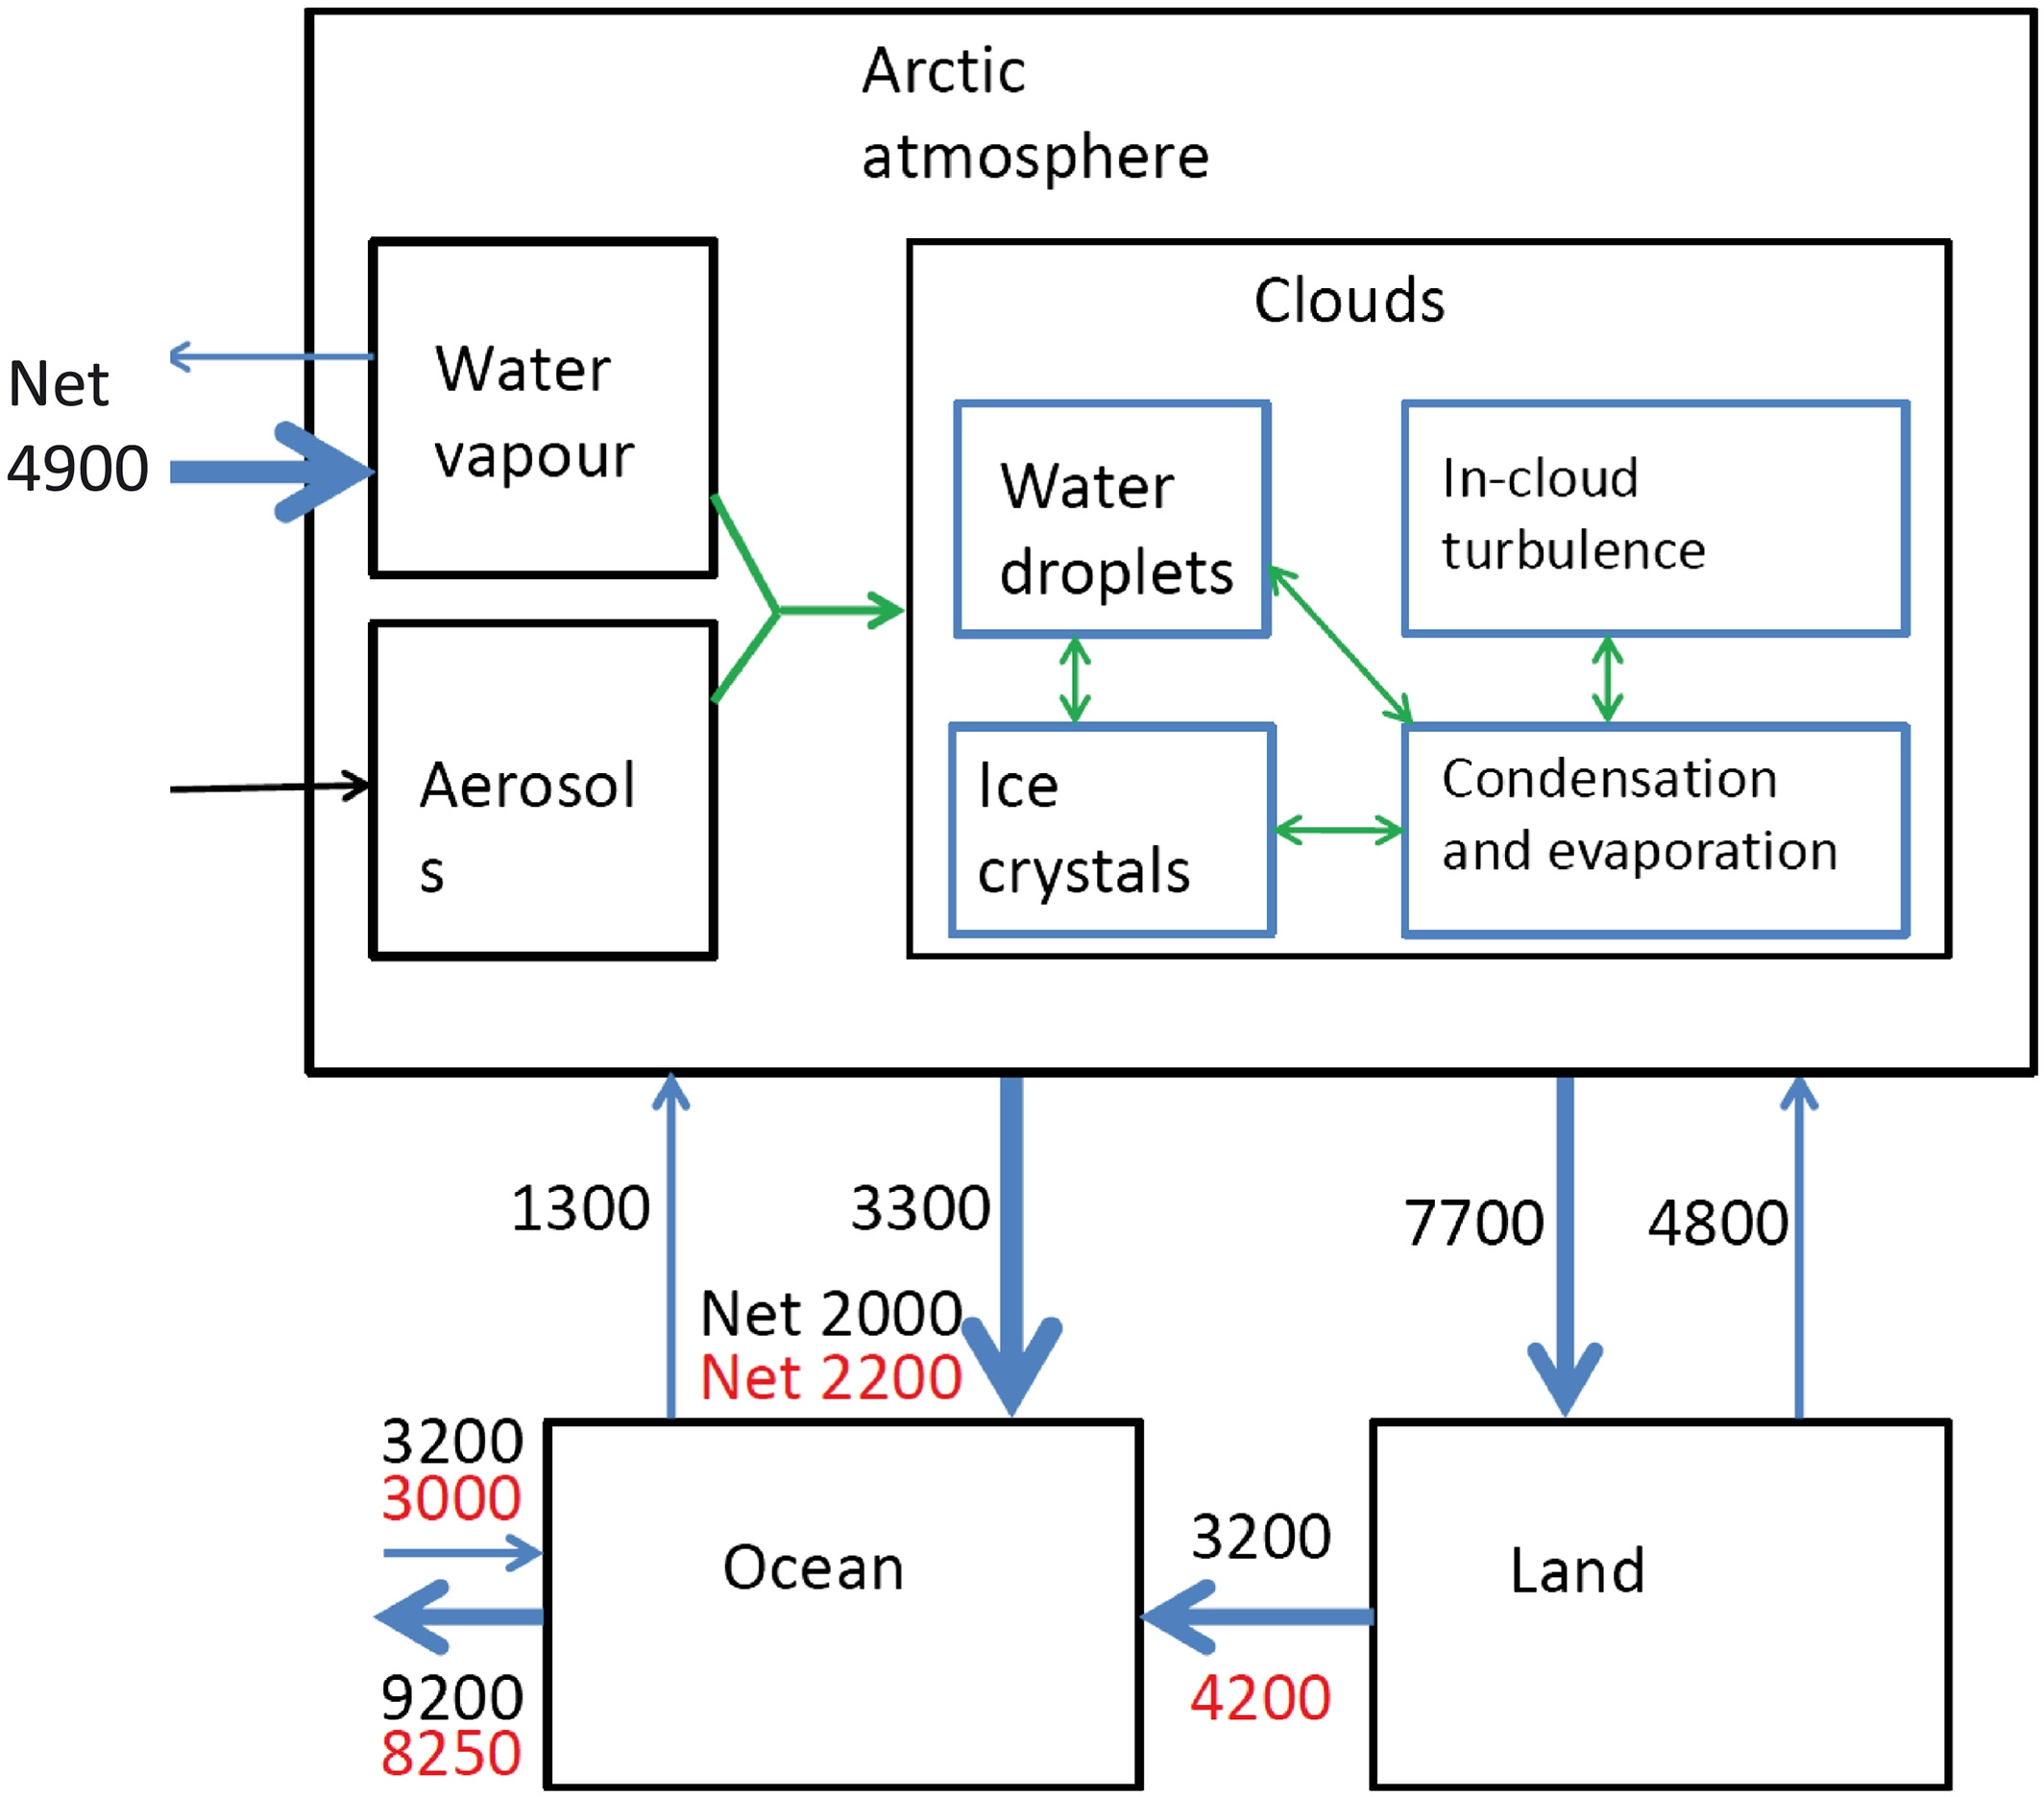
\includegraphics[width=0.7\textwidth]{hydological_cycle.png}
\caption{Schematic of the main freshwater components and processes in the Arctic hydrological cycle \cite{vihma2016atmospheric}. The numbers in black show the main freshwater transports in $km^3/yr$ based on \cite{serreze2006large} for 1979-2010, with the numbers in red show the estimates for 2000-2010 from   \cite{haine2015arctic}. }\label{fig:hydro_cycle}
\end{figure}




\subsubsection{Atmospheric moisture }

In the polar regions the atmospheric component of the hydrological cycle is composed of a moisture flux, where precipitation (P) and evaporation (E) converge to give a and net positive precipitation (P-E). The primary input of water into the polar regions is through atmospheric moisture transport. The P-E is generally an input of freshwater from the atmosphere to the ocean \cite{oshima2017atmospheric}. 

Water vapour in the Arctic has a residence time of around a week, compared with a decade for freshwater in the Arctic ocean, with the spatial and temporal distributions of vapour relation to air temperature distributions. As explained in section \ref{cc} the moisture holding capacity of air increases exponentially with air temperature, and therefore total vertically integrated water vapour (TWV) decreases with increase in longitude, from summer to winter and is higher over the open ocean which is warmer than the cyrosphere. As a result clouds are more common over the open ocean than ice, and sparse over the continents. The amount of cloud cover reaches a maximum in the mid latitude Arctic regions in the late summer, and a minimum during the late winter. The occurance of water vapour and clouds in the Arctic is due to local evaporation and evapotranspiration and condensation due to transport to lower latitudes. The seasonal cycles of P-E over the regions are governed by cyclone cycles where interannual variations are determines by the Arctic Oscillation. 


Atmospheric moisture is composed of water vapour which is the source of cloud and fog formation, which affect radiative transfer, evaporation and condensation, where relative humidity controls cloud formation. During cloud formation, the level where saturation is reached depends on the vertical temperature profiles and specific humidity. As the volume of unsaturated air cools, it's relative humidity increases since the ability for air to hold vapour decreases with temperature, the air temperature inversion generally occurs between 1-1.5 km but this has strong seasonal and spatial variation. 

Changes in specific humidity also effect longwave and shortwave radiative transfer in the atmosphere, where humid air emits more longwave radiation than dry air due to its humidity and temperature. 


Other sources of atmospheric moisture in the Arctic is transported from lower latitudes, driven by the north-south gradient in air specific humidity and is affected by large-scale circulation patterns such as planetary waves, subtropical jet stream, the Polar front jet stream, storm track, Jalley, Ferrel and Polar cells. These phenomenon are split up into mean meridional circulation, stationary eddies and transient eddies. 


%add more detail here https://agupubs.onlinelibrary.wiley.com/doi/10.1002/2015JG003132

\paragraph{Cloud cover}
Cloud cover is difficult to determine in the Arctic due to temporal and spatial limitations, with data indicating that the Arctic has an annual cycle of cloudiness ranging from 40-70\% in winter to 80-95\% in summer. Low clouds and fog dominate and predominantly have a warming effect on the surface, especially over the ice covered part of the Arctic Ocean. Cloudy conditions are often related to a warmer free troposphere, as cloudy episodes are typically associated with advection from lower latitudes. 


\paragraph{Precipitation}
In winter the spatial distributions of precipitation and evaporation are dominated by the difference between large values over the open seas and low values over snow/ice-covered sea and land areas. In summer, both precipitation and evaporation over Arctic land areas, except Greenland, exceed the values over sea areas north of 70$^{\circ}$N and are comparable to those at lower latitudes. Precipitation and evaporation/evapotranspiration affect the ocean and terrestrial freshwater budgets, the surface albedo and energy budget, and the mass balance of ice sheets, glaciers, and sea ice. Arctic ocean freshening occurs during the snow and ice melt in the summer, with river discharge also resulting in freshening. Over continents, in most of the Arctic river catchment, net precipitation is stored as snow for half a year or more

The reduction and increase of snow cover over the seasonal cycle effects the albedo of the surface. Snow and ice surface albedo depending on several factors, such as the snow wetness, temperature, density, grain structure, impurities, melt ponds, and surface slope. 

\subsubsection{Cryosphere}
define the crosphere 

Of the components which constitute the Arctic environment, the cryosphere is the most sensitive to the effects of the changing climate \cite{rinke2019trends}. The cyrosphere, which is the ice component of the Earth's surface is closely linked with terrestrial and freshwater ecosystems, making it a crucial component within the Arctic system.

The changing cyrosphere effects the overall hydrological cycle within the Arctic, contributing to the warmer and wetter conditions which have been seen in recent years. The cryosphere amplifies climate change through snow, ice and permafrost feedbacks. 

Crysopheric changes are detailed more closely in section \ref{local} below. 

\paragraph{Sea ice}
Sea ice amount has a natural fluctuation within the Arctic climate system throughout the year, with coverage between 5 and 6 million $km^2$ at the end of the summer to 14 million $km^2$ at the end of winter. 

\paragraph{Snow cover}
In the Arctic, snow can account for up to 80\% of total precipitation. Snow extent and fall is crucial to the hydrological cycle, where its albedo affects surface radiation balances and water budgets and the habitat of land and water biota. Snow is an insulator affecting the thermal balances of the ground and permafrost distribution. 


\paragraph{Glaciers and Ice Sheets}
The majority of the total volume of ice in the Arctic is contained in Greenland, with Canada having major ice caps and glaciers in the high Arctic and Yukon. 

\paragraph{Permafrost}\label{permafrost}

The frozen component of the ground, such as rock and ice which remains permanently frozen is known as permafrost. Permafrost is composed of an upper layer which thaws during the summer and freezes again during the autumn/winter, which is known as the active layer. Permafrost covers approximately 25\% of and in the Northern Hemisphere and contains twice as much carbon as the atmosphere. 

%Regions where frozen soil melts can be dangerous and deterimental to local communities. 

Frozen ground plays a very important role in the hydrological cycle due to its influence on runoff, groundwater storage, purity and flow and overall influences on water filtration. When active-layers thicken this can lead to 
increased filtration, larger amounts of groundwater storage, increase in base flow (the flow that is sustained between precipitation events) and lower spring runoff. This increase in liquid water is a positive feedback which drives increased rain precipitation, permafrost and glacial melt. 



\paragraph{River and lake ice}
The timing and severity of hydrological extremes in Northern climate systems are heavily affected by freshwater ice, with river ice being a crucial component in river ecology.




\section{Characterizing Arctic change}
Climate sensitivity 

Arctic climate change is mainly characterized by a warmer and wetter atmosphere. This is due to the overall global increase in temperature, in addition to poleward energy transport, snow and ice albedo feedbacks, loss of sea ice and snow, the confining of warming to the near-surface in the polar atmosphere, moisture transport and water-vapor radiative feedback which all contribute to amplification \cite{serreze2011processes}. These are combined effects which differ between the hemispheres, and are more severe in the Arctic as explained in section \ref{arctic change}.

{\color{blue}how do these changes matter and how do they differ?}

The main question and discussion regarding Arctic moistening and the increase in the overall precipitation in the region as the Arctic warms is; is the increased precipitation from local changes to the hydrological cycle (ie sea ice melt) or is it from remote sources (thus transported from lower latitudes). As explained in \cite{bintanja2014future} finding the answer to this question is important for two main reasons. The first; if the precipitation increase is largely linked to local changes, that means that the increase is due to increased warming and melt of sea ice and glaciers in the Arctic region. Since the increased melting directly contributes to increased precipitation, little changes will occur to the overall salinity of the ocean, since evaporation and precipitation will for the most part, cancel out. This is important when we think of impacts related to freshening, such as the slowing down of the AMOC. The second; if the increased precipitation is from remote changes, this means that there is an increased magnitude and frequency of meridional transport of water vapour to the Arctic, related to more remote evaporation sources. Local and remote changes exhibit different seasonal cycles, and therefore whichever dominates will have different impacts on the local hydrology and ecology of the region.


\section{Local changes}\label{local}
The amount of moisture in the Arctic is determined by the rates of local evaporation and moisture transport from lower latitudes.

\subsection{Local temperature change}\label{local_temp}
The increase in Arctic annual mean surface temperature (land and ocean) between 1971 and 2019 was three times higher than the increase in the global average during the same period \cite{AMAP}. Newer studies estimate that this change is 4 times the amount \cite{rantanen2022arctic}. These temperature increases are driving ice losses and changes in moisture transport.


show a table showing which paper, what methods, for what amount of temperature change


This increased temperature results in changes in humidity as the warmer air can hold more moisture section \ref{cc}. 

\subsection{Local humidity change}
The increased temperature discussed in section \ref{local_temp} means that the Arctic air can hold more moisture in accordance with the Clausius-Clapeyron relation section \ref{cc}. 


Moist energy balance models and general circulation models show 1.8 times more warming than dry models, due to the warming effect of latent heat transport \cite{feldl2021polar}. This increased humidity results in increased precipitation, further temperature increases and sea ice losses \cite{mccrystall2021new}. 


\subsection{Local precipitation changes}
A large percentage of Arctic precipitation changes are related to local changes in evaporation and temperature, directly related to humidity and sea ice. There is both an increase in the frequency and magnitude of events, with extreme events becoming more common, in addition to the day of first snow melt coming earlier with each year. The phase of precipitation is changing too, with the end of century predictions leaning towards a rain as opposed to snow dominated Arctic. 


While moisture intrusions are important (as will be discussed below) end-of-century humidity recycling is projected to account for 60-64\% of precipitation in the Arctic \cite{ford2022arctic}.

The Arctic region is seeing a change in precipitation patterns, with regions of the high Arctic being dry in the past becoming wetter in the future. 



\subsection{Cyrosphere}
\subsubsection{Snow cover}
Between 1972 and 2003 the average snow cover extent in the Northern Hemisphere decreased by around 10\%. The projected increases in Arctic temperature will decrease the length of time available for snow to accumulate in winter, affecting the winter snow melt, which is a major component of the hydrological cycle. 


\subsubsection{Glaciers}
Glaciers and ice-caps across the Arctic show a general retreat among glacier fronts and overall volume decreases since the 1920s.

\subsubsection{Permafrost}
Changes in depth and extent of the active layer is an area of continuous study in relation to amplification. This has grown deeper at many sites since the 1990s and landscape observations also show considerable thaw across the Arctic. The largest magnitude of thaw is occurring in the WCA. Melting permafrost results in an increase of carbon into the atmosphere, a positive feedback with overall planetary warming.  


\subsection{Sea ice \& Ocean interactions}
The warming atmosphere of the Arctic is resulting in more and more sea ice melting each year. There has been a considerable loss in sea ice extent since 1979, with a yearly decrease in sea ice expected to continue with the increase in CO2 in the atmosphere \cite{dai2019arctic}. Some studies are predicting an ice free summer Arctic before the mid-century unless there is a rapid reduction in greenhouse gas emissions \cite{notz2018trajectory}. The annual average of sea ice in the Northern Hemisphere decreased by about 7.4\% between 1978 and 2003. 



Overall with warming temperatures, ice has less time to form which makes it thinner and causes it to melt earlier. This allows for stronger heat transfer from the ocean to the atmosphere. 

Sea ice melt is an example of a positive-feedback, where increased temperatures cause melting, which reduce albedo, which result in more heat uptake, and the cycle amplifies. In some cases, this melting results in low-lying clouds which have an albedo similar to ice and therefore the feedback is more muted. 

This increased melting is resulting in there being more available moisture in the air, and thus the humidity of the Arctic increasing. The increase in the amount of open water results in more surface area for evaporation and local moisture recycling. 

Previous work investigating Arctic amplification focused entirely on sea ice losses \cite{serreze2009emergence}. While sea ice losses are extremely important, they are not the only mechanism which is contributing to the changing Arctic.  Some work has shown that in aquaplanet models, with no sea ice, Arctic amplification still occurs \cite{russotto2020polar}.

As mentioned in section \ref{local_temp}, winter warming in the Arctic is more severe than that in the summer, with this change being attributed to sea ice changes.

Sea ice changes are mainly being forced by changes in the summer climate ???.

\subsubsection{Ice, leads and polynas}
 Due to a large amount of evaporation from leads and polynyas, the near-surface air humidity over Arctic sea ice is generally close to saturation concerning the ice phase and therefore sublimation is weak \cite{andreas2002near}. 
 
 Leads are large fractures within an expanse of sea ice, where a linear area of open water is present, and often used for transport. They can vary in width from meters to hundreds of meters. Polynyas are areas of open water surrounded by sea ice.



\subsection{The influence of land interactions}
Evapotranspriation changes 
melting glaciers 

Vegetation

melting permafrost 


\section{Remote changes}\label{remote}
\subsection{Moisture transport and intrusions}
Meridional moisture transport is the transport from lower latitudes to upper latitudes and vise versa. Meridional transports differ between seasons and are strong sources of atmospheric moisture from lower latitudes. 

not much agreement here 

Medidional moisture transport is driven by the north-south gradient of air-specific humidity and are affected by large-scale circulation patterns such as planetary waves, subtropical jet stream, the Polar front jet stream and storm tracks \cite{gimeno2019atmospheric}. These phenomena are split up into mean meridional circulation, stationary eddies and transient eddies. 

There has been an overall increase in atmospheric and ocean heat transport to the poles due to changes in the transport of latent energy (moisture) and dry static energy (the sum of sensible and potential energy) by atmospheric circulations \cite{mcgraw2020changes}. Particularly there are large increases seen over the Atlantic sector of the Arctic \cite{dufour2016atmospheric}, with little analysis of moisture transport over the Western Canadian Arctic. 

\subsection{Poleward heat transport}
\subsection{Storm tracks and blocking}
\subsection{Aerosols}
see figure 1 \cite{vihma2016atmospheric}
\section{Knowledge gaps}
\section{Conclusion}






 \bibliography{../mybib}{}
\bibliographystyle{apalike}

\end{document}


